\documentclass[12pt,letterpaper]{exam}
\usepackage[lmargin=1in,rmargin=1in,tmargin=1in,bmargin=1in]{geometry}
\usepackage{../style/exams}

% -------------------
% Course & Exam Information
% -------------------
\newcommand{\course}{MAT 108: Exam 2}
\newcommand{\term}{Fall -- 2021}
\newcommand{\examdate}{11/18/2021}
\newcommand{\timelimit}{85 Minutes}

\setbool{hideans}{false} % Student: True; Instructor: False

% -------------------
% Content
% -------------------
\begin{document}

\examtitle
\instructions{Write your name on the appropriate line on the exam cover sheet. This exam contains \numpages\ pages (including this cover page) and \numquestions\ questions. Check that you have every page of the exam. Answer the questions in the spaces provided on the question sheets. Be sure to answer every part of each question and show all your work. If you run out of room for an answer, continue on the back of the page --- being sure to indicate the problem number.} 
\scores
\bottomline
\newpage

% ---------
% Questions
% ---------
\begin{questions}

% Question 1
\newpage
\question[10] Find the maximum and minimum values (if they exist) for the function $z= 5x_1 - 3x_2$ for the region shown below. 
	\[
	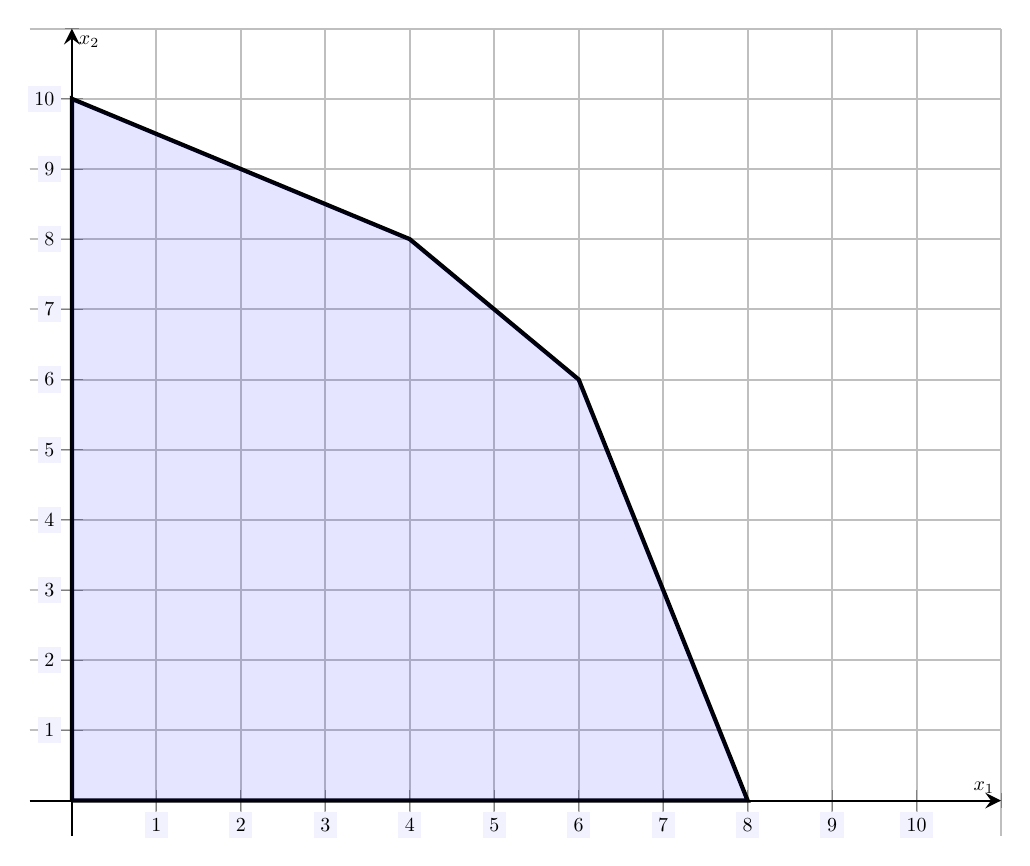
\begin{tikzpicture}[scale=1.8,every node/.style={scale=0.4}]
	\begin{axis}[
	grid=both,
	axis lines=middle,
	ticklabel style={fill=blue!5!white},
	xmin= -0.5, xmax=11,
	ymin= -0.5, ymax=11,
	xtick={-1,0,1,...,10},
	ytick={-1,0,1,...,10},
	minor tick = {-11,...,11},
	xlabel=\(x_1\),ylabel=\(x_2\),
	]
	\draw[line width=0.03cm] (0,0) -- (0,10) -- (4,8) -- (6,6) -- (8,0) -- (0,0);
	\draw[line width=0.01cm,fill= blue,opacity=0.1] (0,0) -- (0,10) -- (4,8) -- (6,6) -- (8,0) -- (0,0);
	\end{axis}
	\end{tikzpicture}
	\] \pspace

{\itshape By the Fundamental Theorem of Linear Programming, because this region is nonempty and bounded, the function $z(x_1, x_2)$ must have a maximum and a minimum and that these extrema occur at corner points for the region. Examining the graph, we see that the corner points are $(0, 0)$, $(0, 10)$, $(4, 8)$, $(6, 6)$, and $(8, 0)$. Then\dots\par
	\begin{table}[!ht]
	\centering
	\begin{tabular}{l|l}
	Point & $z= 5x_1 - 3x_2$ \\ \hline
	$(0, 0)$ & $5(0) - 3(0)= 0 - 0= 0$ \\
	$(0, 10)$ & $5(0) - 3(10)= 0 - 30= -30$ \\
	$(4, 8)$ & $5(4) - 3(8)= 20 - 24= -4$ \\
	$(6, 6)$ & $5(6) - 3(6)= 30 - 18= 22$ \\
	$(8, 0)$ & $5(8) - 3(0)= 40 - 0= 40$
	\end{tabular}
	\end{table} \par
Therefore, the maximum value of $z$ is 40 occurring at $(8, 0)$ while the minimum value of $z$ is $-30$ occurring at $(0, 10)$. 
	\[
	\boxed{%
	\begin{aligned}
	\max\colon& z(8,0)= 40 \\
	\min\colon& z(0,10)= -30
	\end{aligned}%
	}
	\]
}





% Question 2
\newpage
\question[10] Find the tableau corresponding to the standard form of the following constrained maximization problem:
	\[
	\begin{aligned}
	\max z= 2x_1 - x_2& + 5x_3 \\
	2x_1 - x_2 + 3x_3&\leq 5 \\
	x_1 - 4x_2 - x_3&\leq 3 \\
	x_1 - x_2 - x_3&\geq 1 \\
	x_1, x_2, x_3 \geq 0
	\end{aligned}
	\] \pspace

{\itshape First, we negate the third inequality so that we have the proper inequalities. 
	\[
	\begin{aligned}
	2x_1 - x_2 + 3x_3&\leq 5 \\
	x_1 - 4x_2 - x_3&\leq 3 \\
	-x_1 + x_2 + x_3&\leq -1
	\end{aligned}
	\]
Now we introduce slack variables $s_1, s_2, s_3$ to obtain equalities. 
	\[
	\begin{aligned}
	&2x_1 &-& &x_2& &+& &3x_3& &+& &s_1&&&&&=& 5 \\
	&x_1 &-& &4x_2& &-& &x_3& &+& &&&s_2&&&=& 3 \\
	-&x_1 &+& &x_2& &+& &x_3& &+& &&&&&s_3&=& -1
	\end{aligned}
	\]
Finally, moving everything to the left side in $z= 2x_1 - x_2 + 5x_3$, we have $z - 2x_1 + x_2 - 5x_3= 0$. This yields an initial tableau of\dots \par
	\begin{table}[!ht]
	\centering
	\framebox{%
	\begin{tabular}{rrrrrr|r}
	$2$ & $-1$ & $3$ & $1$ & $0$ & $0$ & $5$ \\
	$1$ & $-4$ & $-1$ & $0$& $1$ & $0$ & $3$ \\
	$-1$ & $1$ & $1$ & $0$ & $0$& $1$ & $-1$ \\ \hline
	$-2$ & $1$ & $-5$ & $0$ & $0$& $0$ & $0$
	\end{tabular}
	}
	\end{table} \par
One could also not change the third inequality and instead introduce slack variables $s_1, s_2$, as before, and surplus variable $s_3$:
	\[
	\begin{aligned}
	&2x_1 &-& &x_2& &+& &3x_3& &+& &s_1&&&&&=& 5 \\
	&x_1 &-& &4x_2& &-& &x_3& &+& &&&s_2&&&=& 3 \\
	&x_1 &-& &x_2& &-& &x_3& &-& &&&&&s_3&=& 1
	\end{aligned}
	\]
This then leads to an initial tableau of\dots \par
	\begin{table}[!ht]
	\centering
	\begin{tabular}{rrrrrr|r}
	$2$ & $-1$ & $3$ & $1$ & $0$ & $0$ & $5$ \\
	$1$ & $-4$ & $-1$ & $0$& $1$ & $0$ & $3$ \\
	$1$ & $-1$ & $-1$ & $0$ & $0$& $-1$ & $1$ \\ \hline
	$-2$ & $1$ & $-5$ & $0$ & $0$& $0$ & $0$
	\end{tabular}
	\end{table}
}





% Question 3
\newpage
\question[10] Find the dual problem to the standard form of the following constrained minimization problem: 
	\[
	\begin{aligned}
	\min z= 4x_1 + 5x_2& + 6x_3 \\
	3x_1 - x_2 + 5x_3&\geq 6 \\
	-x_1 + 4x_2 - 2x_3&\leq 4 \\
	6x_1 + x_2 - 8x_3&\geq 7 \\
	x_1, x_2, x_3 \geq 0
	\end{aligned}
	\] \pspace

{\itshape First, we multiply the second inequality by $-1$ to obtain the correct inequality for a standard form minimization problem. 
	\[
	\begin{aligned}
	3x_1 - x_2 + 5x_3&\geq 6 \\
	x_1 - 4x_2 + 2x_3&\geq -4 \\
	6x_1 + x_2 - 8x_3&\geq 7	
	\end{aligned}
	\]
Next, we form the matrix of the constraints along with the objective function:
	\[
	\begin{pmatrix*}[r]
	3 & -1 & 5 & 6 \\
	1 & -4 &  2 & -4 \\
	6 & 1 & -8 & 7 \\
	4 & 5 & 6 & 0 
	\end{pmatrix*}
	\]
We take the transpose of this matrix. 
	\[
	\begin{pmatrix*}[r]
	3 & 1 & 6 & \phantom{-}4 \\
	-1 & -4 & 1 & 5 \\
	5 & 2 & -8 & 6 \\
	6 & -4 & 7 & 0 
	\end{pmatrix*}
	\]
This corresponds to the following standard form maximization problem:
	\[
	\begin{aligned}
	\max w= 6y_1 - 4y_2& + 7y_3 \\
	3y_1 + y_2 + 6y_3&\leq 4 \\
	-y_1 - 4y_2 + y_3&\leq 5 \\
	5y_1 + 2y_2 - 8y_3&\leq 6 \\
	y_1, y_2, y_3 \geq 0
	\end{aligned}
	\] 
}





% Question 4
\newpage
\question[10] Below is the final tableau for a standard maximization problem. Find the solution to this maximization problem and find the maximum value for the function.
	\begin{table}[!ht]
	\centering
	\begin{tabular}{rrrrrrr}
	$0$ & $0.794$ & $1$ & $0.032$ & $0$ & $0.022$ & $8.868$ \\
	$0$ & $-22.608$ & $0$ & $0.038$ & $1$ & $-0.429$ & $211.935$ \\
	$1$ & $-0.195$ & $0$ & $-0.026$ & $0$ & $0.028$ & $0.699$ \\
	$0$ & $33.916$ & $0$ & $0.422$ & $0$ & $0.833$ & $212.347$
	\end{tabular}
	\end{table}

{\itshape To help read the tableau, we insert the variables corresponding to the columns as well as our dividers: \par
	\begin{table}[!ht]
	\centering
	\begin{tabular}{rrrrrrr}
	{\scriptsize$x_1$} & {\scriptsize$x_2$} & {\scriptsize$x_3$} & {\scriptsize$s_1$} & {\scriptsize$s_2$} & {\scriptsize$s_3$} & \\
	$0$ & $0.794$ & $1$ & $0.032$ & $0$ & \multicolumn{1}{r|}{$0.022$} & $8.868$ \\
	$0$ & $-22.608$ & $0$ & $0.038$ & $1$ & \multicolumn{1}{r|}{$-0.429$} & $211.935$ \\
	$1$ & $-0.195$ & $0$ & $-0.026$ & $0$ & \multicolumn{1}{r|}{$0.028$} & $0.699$ \\ \hline
	$0$ & $33.916$ & $0$ & $0.422$ & $0$ & \multicolumn{1}{r|}{$0.833$} & $212.347$ 
	\end{tabular}
	\end{table} \par
Reading the pivot columns, i.e. the columns with $1$'s, we see that $x_1= 0.699$, $x_3= 8.868$, $s_2= 211.935$. The remaining variables and slack variables must then be zero. So we have\dots
	\[
	(x_1, x_2, x_3, s_1, s_2, s_3)= (0.699, 0, 8.868, 0, 211.935, 0)
	\]
}





% Question 5
\newpage
\question[10] Suppose a researcher wants to create a linear model to predict a certain crop's average growth, $g$, in cm using the average number of hours of sunlight, $h$, the crops receive per day. They sample 61 different fields and collect the following data:
	\[
	\begin{aligned}
	\overline{h}&= 10 & \overline{g}&= 120 \\
	s_h^2&= 4 & s_g^2&= 64 \\
	n&= 61 & r&= 0.5
	\end{aligned}
	\] \pspace

\begin{parts}
\part Find the linear regression model to predict the growth rate using the number of hours of sunlight. \pvspace{0.3cm}

{\itshape First, we have $s_h= \sqrt{4}= 2$ and $s_g= \sqrt{64}= 8$. We have
	\[
	\begin{aligned}
	b_1&= r\, \dfrac{s_g}{s_h} &\qquad b_0&= \overline{g} - \overline{h}\, b_1 \\
	b_1&= 0.5 \cdot \dfrac{8}{2} & b_0&= 120 - 10(2) \\
	b_1&= 2 & b_0&= 100
	\end{aligned}
	\]
But then we have regression model $\widehat{g}= 2h + 100$.} \pvspace{0.3cm}

\part Predict the average growth of crops that receive an average of 9~hours of sunlight. \pvspace{0.5cm}

{\itshape
	\[
	\widehat{g}= 2(9) + 100= 18 + 100= 118 \text{ cm}
	\]
} \pvspace{0.5cm}

\part Suppose that a crop which receives an average of 9~hours of sunlight per day grows an average of 110~cm. Find the residual for the model's prediction. Is the prediction an under or over prediction? \pvspace{0.3cm}

{\itshape
	\[
	e_i= g_{\text{obs}} - \widehat{g}= 110 - 118= -8 \text{ cm}
	\]
Because $e_i < 0$, the model is an overprediction. Equivalently, because $118 > 110$, the model is an overprediction.} \pvspace{0.3cm}

\part Does the average growth rate of the crops appear to be strongly correlated with the average number of hours of sunlight they receive per day? Explain. \pvspace{0.3cm}

{\itshape No, there does not appear to be a strong relationship between the two based on the given data/model. The $r$-value for this model is $0.5$ (which gives $r^2$ value $0.24$), which indicates a poor predictive relationship.}
\end{parts}





% Question 6
\newpage
\question[10] Researchers collected data on the number of running shoes sold based on the price of the shoe. Plotted below is a linear model fitted to a scatterplot of the data collected by the researchers:
	\begin{figure}[!ht]
	\centering
	\includegraphics[width=0.65\textwidth]{linreg.png}
	\end{figure} 

\begin{parts}
\part Which of the following is the most likely equation for the linear model?
	\begin{enumerate}[(i)]
	\item \usol{0.5cm}{\phantom{a}}: $\widehat{y}= 2.89x + 533$ 
	\item \usol{0.5cm}{\phantom{a}}: $\widehat{y}= -2.99x + 601.37$ 
	\item \usol{0.45cm}{\cmark}: $\widehat{y}= 797.27 - 2.97x$ 
	\item \usol{0.5cm}{\phantom{a}}: $\widehat{y}= 353.70x - 67.33$ 
	\end{enumerate} \pvspace{0.2cm}

\part Which of the following is the most likely $r$ value for this model?
	\begin{enumerate}[(i)]
	\item \usol{0.45cm}{\cmark}: $r= -0.9803$ 
	\item \usol{0.5cm}{\phantom{a}}: $r= 0.9803$ 
	\item \usol{0.5cm}{\phantom{a}}: $r= -0.2407$ 
	\item \usol{0.5cm}{\phantom{a}}: $r= 0.2407$ 
	\end{enumerate} \pvspace{0.2cm}

\part Approximately how many shoes does the model predict will be sold if the price of the shoe is \$80? \pvspace{0.5cm}

{\itshape Examining the graph, the model predicts a shoe price of \$80 leads to approximately 550 shoes (exact value 559) being sold.} \pvspace{0.5cm}

\part Should the model be used to predict the number of shoes that will sell for a shoe priced at \$200? Explain. \pvspace{0.3cm}

{\itshape No, the model should not be used to predict shoe sales for a price of \$200. The model was constructed using values only between approximately \$10 and \$120. A shoe price of \$200 is `far' outside this range and one should not extrapolate so far (without good reason).}
\end{parts}





% Question 7
\newpage
\question[10] Robyn Banks is opening a savings account to create a travel fund to surprise her niece with after her high school graduation (when she turns 18). Suppose the account accrues interest at a 1.2\% annual interest rate, compounded quarterly. \pspace
        \begin{parts}
        \part How much should she put into the account to have \$3,600 set aside for her newborn niece's high school graduation? \pvspace{0.3cm}

{\itshape
\begin{minipage}[c]{0.45\textwidth}
	\[
	\begin{aligned}
	F&= 3600 \\
	r&= 0.012 \\
	k&= 4 \\
	n&= 18 \cdot 4= 72
	\end{aligned}
	\]
\end{minipage}%
\begin{minipage}[b]{0.45\textwidth}
	\[
	\begin{aligned}
	P&= \dfrac{F}{\left(1 + \dfrac{r}{k} \right)^n} \\
	P&= \dfrac{3600}{\left(1 + \dfrac{0.012}{4} \right)^{72}} \\
	P&= \dfrac{3600}{1.2407} \\
	P&= \$2901.59
	\end{aligned}
	\]
\end{minipage}
} \pvspace{0.6cm}

        \part If she places \$800 in the account, how much money will she be giving her niece? \pvspace{1.2cm}

{\itshape
\begin{minipage}[c]{0.45\textwidth}
	\[
	\begin{aligned}
	P&= 800 \\
	r&= 0.012 \\
	k&= 4 \\
	n&= 18 \cdot 4= 72
	\end{aligned}
	\]
\end{minipage}%
\begin{minipage}[b]{0.45\textwidth}
	\[
	\begin{aligned}
	F&= P \left( 1 + \dfrac{r}{k} \right)^n \\
	F&= 800 \left( 1 + \dfrac{0.012}{4} \right)^{72} \\
	F&= 800(1.2407) \\
	F&= \$992.56
	\end{aligned}
	\]
\end{minipage}
} \pvspace{1.2cm}

        \part Assuming she places \$800 into the account, how long until the account has \$1,100? \pvspace{0.3cm}
        
{\itshape Note that because the interest is compounded four times per year, the number of years is one-fourth the number of compounds. \par
\begin{minipage}[c]{0.45\textwidth}
	\[
	\begin{aligned}
	F&= 1100 \\
	P&= 800 \\
	r&= 0.012 \\
	k&= 4 
	\end{aligned}
	\]
\end{minipage}%
\begin{minipage}[b]{0.45\textwidth}
	\[
	\begin{aligned}
	t&= \dfrac{1}{4} \cdot n= \cdot \dfrac{\log(F/P)}{\log\left( 1 + \dfrac{r}{k} \right)} \\
	t&= \dfrac{1}{4} \cdot \dfrac{\log(1100/800)}{\log( 1 + \frac{0.012}{4} )} \\
	t&= \dfrac{1}{4} \cdot \dfrac{0.318454}{0.00299551} \\
	t&= 26.58 \text{ years}
	\end{aligned}
	\]
\end{minipage}
}
	\end{parts} 





% Question 8
\newpage
\question[10] Hugh Nowes and his wife Ivana purchase a \$100,000 home, making a \$20,000 down payment. They get a mortgage for the remaining balance at an annual interest rate of 8.5\% compounded monthly that will be repaid in monthly installments over a 20~year payment. \pspace
        \begin{parts}
        \part What are the monthly payments? \pvspace{0.3cm}

{\itshape
\begin{minipage}[c]{0.45\textwidth}
	\[
	\begin{aligned}
	P&= 80000 \\
	r&= 0.085 \\
	k&= 12 \\
	n&= 12 \cdot 20= 240 
	\end{aligned}
	\]
\end{minipage}%
\begin{minipage}[b]{0.45\textwidth}
	\[
	\begin{aligned}
	R&= \dfrac{P}{\dfrac{1 - \left( 1 + \dfrac{r}{k} \right)^{-n}}{r/k}} \\[0.3cm]
	R&= \dfrac{80000}{\dfrac{1 - \left( 1 + \dfrac{0.085}{12} \right)^{-240}}{0.085/12}} \\[0.3cm]
	R&= \dfrac{80000}{\dfrac{1 - 0.183782}{0.00708333}} \\[0.3cm]
	R&= \dfrac{80000}{115.231} \\[0.3cm]
	R&= \$694.26
	\end{aligned}
	\]
\end{minipage}
} \pvspace{0.5cm}

        \part How much is owed after 10~years? \pvspace{0.3cm}

{\itshape
\begin{minipage}[c]{0.45\textwidth}
	\[
	\begin{aligned}
	R&= 694.26 \text{ (above)} \\
	r&= 0.085 \\
	k&= 12 \\
	n&= 12 \cdot 20= 240 \\
	m&= 10 \cdot 12= 120 
	\end{aligned}
	\]
\end{minipage}%
\begin{minipage}[b]{0.45\textwidth}
	\[
	\begin{aligned}
	P&= R\; \dfrac{1 - \left( 1 + \dfrac{r}{k} \right)^{-(n - m)}}{r/k} \\[0.3cm]
	P&= 694.26 \cdot \dfrac{1 - \left( 1 + \dfrac{0.085}{12} \right)^{-(240 - 120)}}{0.085/12} \\[0.3cm]
	P&= 694.26 \cdot \dfrac{1 - 0.4286975}{0.00708333} \\[0.3cm]
	P&= 694.26 \cdot 80.6545 \\[0.3cm]
	P&= \$55,995.20
	\end{aligned}
	\]
\end{minipage}
}
        \end{parts}





% Question 9
\newpage
\question[10] Sue Donnim places \$2,000 into a portfolio which accrues 4.5\% interest compounded continuously. \pspace
        \begin{parts}
        \part How much money will be in the account after 6~years? \pvspace{2.8cm}

{\itshape
\begin{minipage}[c]{0.45\textwidth}
	\[
	\begin{aligned}
	P&= 2000 \\
	r&= 0.045 \\
	t&= 6
	\end{aligned}
	\]
\end{minipage}%
\begin{minipage}[b]{0.45\textwidth}
	\[
	\begin{aligned}
	F&= Per^{rt} \\[0.3cm]
	F&= 2000\, e^{0.045 \cdot 6} \\[0.3cm]
	F&= 2000\, e^{0.27} \\[0.3cm]
	F&= 2000(1.30996) \\[0.3cm]
	F&= \$2,169.92
	\end{aligned}
	\]
\end{minipage} 
} \pvspace{2.8cm}

        \part What is the effective interest rate? \pvspace{0.3cm}

{\itshape
\begin{minipage}[c]{0.45\textwidth}
	\[
	\begin{aligned}
	r&= 0.045
	\end{aligned}
	\]
\end{minipage}%
\begin{minipage}[b]{0.45\textwidth}
	\[
	\begin{aligned}
	r_{\text{eff}}&= e^r - 1 \\[0.3cm]
	r_{\text{eff}}&= 1.04603 - 1 \\[0.3cm]
	r_{\text{eff}}&= 0.04603
	\end{aligned}
	\]
\end{minipage}
}
        \end{parts}
 
 
 
  

% Question 10
 \newpage
 \question[10] Bill Lowney opens a savings account for retirement into which he places a yearly  \$1,800 deposit. The account has a 7.5\% annual interest rate that is compounded annually. 
        \begin{parts}
        \item How much money will the account have after 30~years? \pvspace{1.4cm}

{\itshape
\begin{minipage}[c]{0.45\textwidth}
	\[
	\begin{aligned}
	R&= 1800 \\
	r&= 0.075 \\
	k&= 1 \\
	n&= 30 
	\end{aligned}
	\]
\end{minipage}%
\begin{minipage}[b]{0.45\textwidth}
	\[
	\begin{aligned}
	F&= R\; \dfrac{\left(1 + \dfrac{r}{k} \right)^n - 1}{r/k} \\[0.3cm]
	F&= 1800\; \dfrac{\left(1 + \dfrac{0.075}{1} \right)^{30} - 1}{0.075/1} \\[0.3cm]
	F&= 1800\; \dfrac{8.75496 - 1}{0.075} \\[0.3cm]
	F&= 1800(103.399) \\[0.3cm]
	F&= \$186,118
	\end{aligned}
	\]
\end{minipage}
} \pvspace{1.4cm}

        \item How much should he deposit each year if he would like \$50,000 in 30~years for his retirement? \pvspace{0.3cm}

{\itshape
\begin{minipage}[c]{0.45\textwidth}
	\[
	\begin{aligned}
	F&= 50000 \\
	r&= 0.075 \\
	k&= 1 \\
	n&= 30 
	\end{aligned}
	\]
\end{minipage}%
\begin{minipage}[b]{0.45\textwidth}
	\[
	\begin{aligned}
	R&= \dfrac{F}{\dfrac{\left( 1 + \dfrac{r}{k} \right)^n - 1}{r/k}} \\[0.3cm]
	R&= \dfrac{50000}{\dfrac{\left( 1 + \dfrac{0.075}{1} \right)^{30} - 1}{0.075/1}} \\[0.3cm]
	R&= \dfrac{50000}{\dfrac{8.75496 - 1}{0.075}} \\[0.3cm]
	R&= \dfrac{50000}{103.399} \\[0.3cm]
	R&= \$483.56
	\end{aligned}
	\]
\end{minipage}
}
        \end{parts} 


\end{questions}
\end{document}